\documentclass[border=5]{standalone}
\usepackage{tikz}
\usetikzlibrary{shadings}
\begin{document}
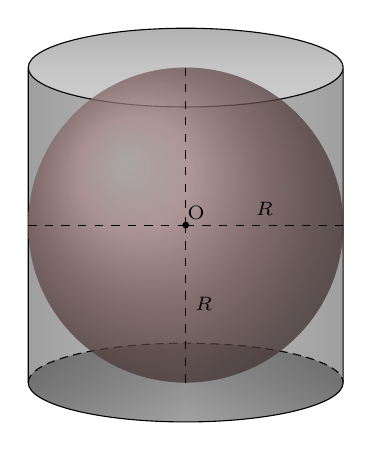
\begin{tikzpicture}
  \fill[top color    = gray!50!black,
        bottom color = gray!10,
        middle color = gray,
        shading      = axis,
        opacity      = 0.25]
    (0,0) circle (2cm and 0.5cm);
  \fill[left color   = gray!50!black,
        right color  = gray!50!black,
        middle color = gray!50,
        shading      = axis,
        opacity      = 0.25]
    (2,0) -- (2,4)  arc (360:180:2cm and 0.5cm)
          -- (-2,0) arc (180:360:2cm and 0.5cm);
  \fill[top color    = gray!90!,
        bottom color = gray!2,
        middle color = gray!30,
        shading      = axis,
        opacity      = 0.25]
    (0,4) circle (2cm and 0.5cm);
  \draw (-2,4) -- (-2,0) arc (180:360:2cm and 0.5cm)
               -- (2,4) ++ (-2,0) circle (2cm and 0.5cm);
  \draw[densely dashed] (-2,0) arc (180:0:2cm and 0.5cm);
  \fill[thick, ball color=red!25, opacity = 0.5] (0,2) circle (2);
  \draw[dashed] (0,0)--(0,2) (0,2)--(0,4);
  \draw[dashed] (-2,2)--(0,2) (0,2)--(2,2);
  \draw[fill=black] (0,2) circle (1pt);
  \node [right] at (-0.1,2.15) {\scriptsize O};
  \node [right] at (0,1) {\scriptsize $R$};
  \node [above] at (1,2) {\scriptsize $R$};
\end{tikzpicture}
\end{document}